%!TEX root = main.tex

\section{Terms} % (fold)
\label{sec:terms}


\begin{description}
    \item[Broadcaster] \hfill \\
    Broadcaster broadcast multiple services inside the local network.
    By listening to a certain port, it could respond to Discoverer's searching query, and return the services list.

    \item[Discoverer] \hfill \\
    Discoverer will keep sending query to certain port to ask for a certain type of services,
    and maintain a local list of services.

    \item[Service] \hfill \\
    Service describes a service with properties.
    It is defined by \emph{type}, \emph{name}, service source \emph{IP}, and \emph{port}.
    All services use a universal unique ID (UUID) as its name.

    \item[RDD] \hfill \\
    RDD is defined as the same with the original paper.
    However, in Spark Driver-less, RDD is only used to record operation lineage to generate Partition lineage.
    It only exists in Client and never be sent to any Worker.
    Every RDD has a \emph{parent} RDD except data source RDDs, and a \emph{get} function for Partition computation.

    \item[Partition] \hfill \\
    Partition is a slice of the RDD, which will be sent to a single worker to compute.
    It has a \emph{part\_id} for the index in the RDD,
    a \emph{uuid} generated from its get function,
    a \emph{parent\_list} of dependent Partitions list,
    and a \emph{func} for computation.

    It is also a Service represents a computed partition,
    with a type of \textit{partition} and its uuid as the name.
    The computed data is called Result.

    \item[Job] \hfill \\
    Job is a Service related to a partition to be computed.
    It has a type of \textit{job}, and use the partition's uuid as its name.

    \item[Worker] \hfill \\
    Worker is a computation process on an arbitrary node.
    It has a Job Discoverer, Job Broadcaster, Partition Discoverer, and Partition Broadcaster.

    It is also a Service with a random uuid as its name.
    But it is only used by Client to optimize \emph{num\_of\_partitions}.

    \item[Client] \hfill \\
    Client is a interactive console for user to compute in the cluster.
    All computation is lazy.
    It creates RDD lineage and transform it into Partition lineage.
    Broadcast target partitions as a Job.
    It keeps discovering Workers in the cluster, and uses the number of workers as \emph{num\_of\_partitions} when it is creating Partition lineage.
\end{description}

Worker and Client's broadcasters and discoveres are shown in Figure~\ref{fig:broadcaster}.

\begin{figure}[htb]
    \centering
    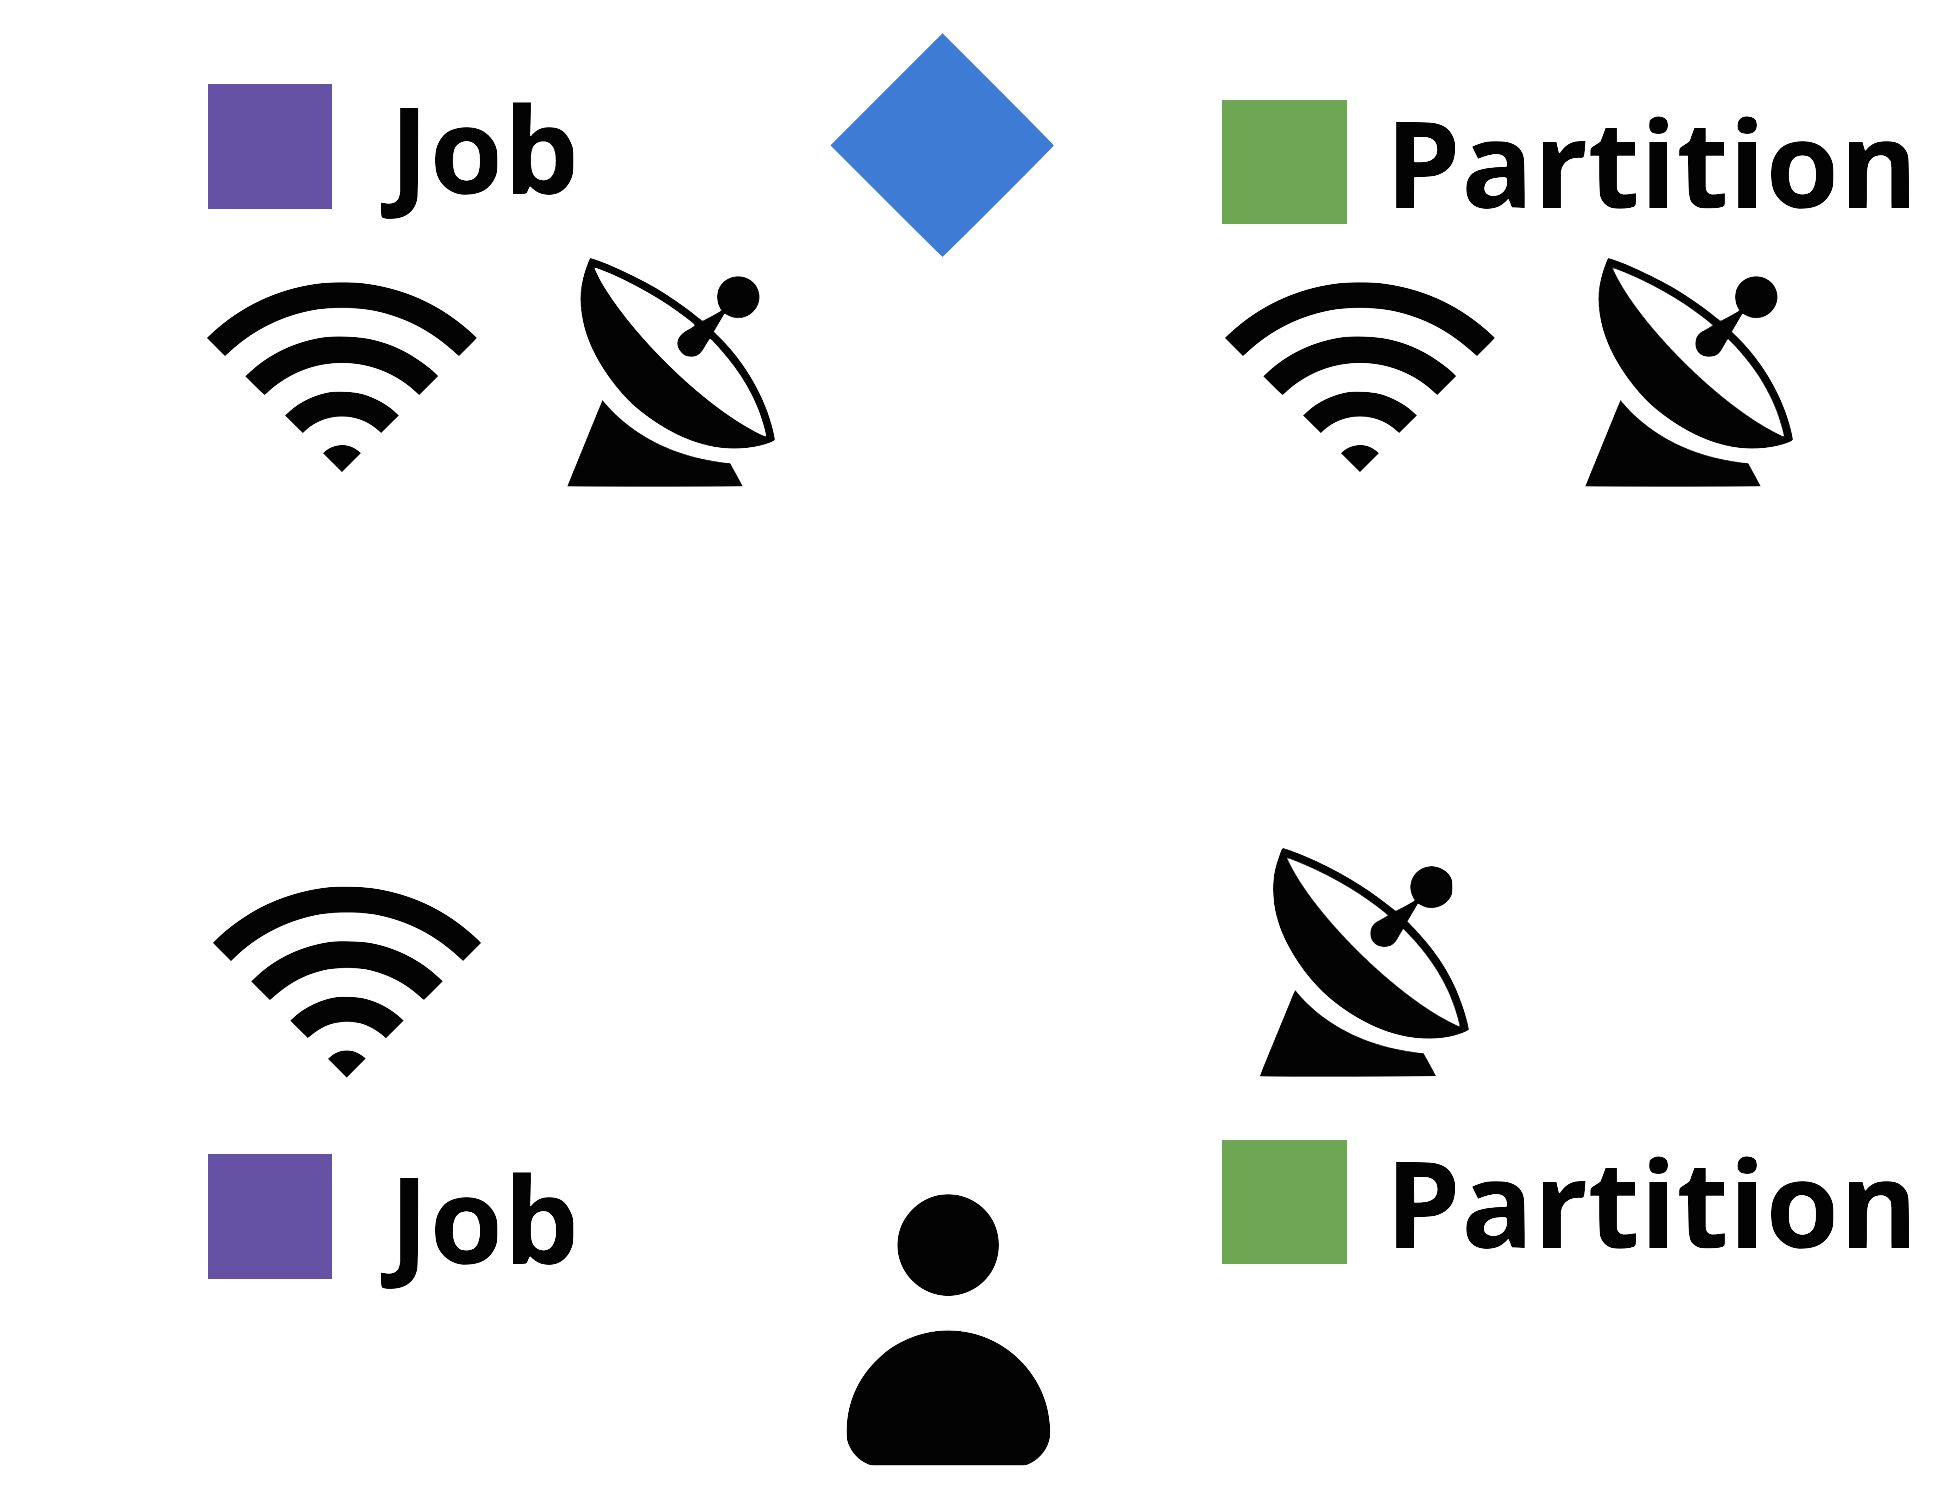
\includegraphics[width=0.5\textwidth]{images/broadcaster.png}
    \caption{Broadcasters and Discoverers}\label{fig:broadcaster}
\end{figure}

% section terms (end)
